\begin{savequote}[8cm]
	\textit{Wir haben gesehn, dass alle Organismen aus wesentlich gleichen Theilen, nämlich aus Zellen zusammengesetzt sind.}
	
	We have seen that all organisms are composed of essentially similar parts, namely, of cells.
	\qauthor{--- \cite{Schwann1839Mikroskopische}}
\end{savequote}

\chapter{\label{ch:2-SDA} Single Cell Transcriptomics}

\minitoc

\section{Introduction}
Cells are the fundamental unit of all living organisms, and with recently developed technologies such as DropSeq it is now possible to perform mRNA sequencing of individual cells for tens of thousands of cells. This enables discovery and characterisation of novel cell types,clues towards gene function via co-expression, as well as characterisation of transcriptional processes such as transcription factor binding.

Here we have generated a dataset of >20,000 cells from both wild type and knockout mice testis, using a matrix factorisation approach to soft cluster cells, infer corresponding co-expressed gene markers, and impute noisy gene expression. This revealed novel marker genes, novel predicted functions for understudied genes, further characterisation of understudied cell types, pathology associated process, and insights into sex chromosome inactivation. We also inferred, \emph{de novo} transcription factor binding motifs, revealing a haploid switch in the types of motifs used.

\vspace{0.7cm}
\begin{framed}
\noindent All experimental work in this chapter was performed by Min Jung and colleges in Don Conrad's group at the University of Washington, St Louis. Much of this chapter has been published as \cite{Jung2019Unified}, on which I am co-first author.
\end{framed}

\section{Experimental Data Generation}

The cells were dissociated by two methods: enzymatic for the first two wild type mice and the spermatogonia, and mechanical for all other samples \parencite{Lima2017Standardized,Jung2019Unified}. The cells were then encapsulated using the DropSeq protocol \parencite{Macosko2015Highly} as described in \cite{Jung2019Unified}. 

The samples generated are as follows:

\begin{itemize}
	\item 11 wild type C57BL/6 mice samples
	\item 3 Hoechst-FACS samples from a 12th wild type (primary spermatocyte (4C), secondary spermatocyte (2C), and spermatid(1C))
	\item 1 sample of FACS sorted spermatogonial cells from 5 wild type C57BL/6 litter mates with GFP tagged Pou5f1 (B6;CBA-Tg(Pou5f1-EGFP)\textsuperscript{2Mnn/J}, from \cite{Szabo2002Allelespecific})
\end{itemize}

In addition to wild type mice four different mutant mice were included:
\begin{itemize}
	\item 6 \textit{Mlh3\textsuperscript{-/-}} mice (B6.129-Mlh3\textsuperscript{tm1Lpkn}/J, \cite{Lipkin2002Meiotic})
	\item 2 \textit{Hormad1\textsuperscript{-/-}} mice (B6;129S7-Hormad1\textsuperscript{tm1Rajk}/Mmjax, \cite{Shin2010Hormad1})
	\item 2 \textit{Cul4a\textsuperscript{-/-}} mice (B6;129-Cul4a\textsuperscript{-/-}, \cite{Yin2011E3})
	\item 2 CNP eGFP BAC TRAP (knockin) C57BL/6 mice (Joseph Dougherty).
\end{itemize}


\section{Data Processing and QC}

The samples were sequenced on either Illumina HiSeq2500 or MiSeq. Reads were mapped to the mouse genome using DropSeq tools provided by Macosko lab (using STAR aligner and GRCm38 release 90).

The resulting cell-gene count matrices were merged (54,251 cells and 38,317 genes) and processed through a series of quality control and normalization steps:

Genes with a UMI count of less than 5 or being expressed in fewer than 5 cells were removed.

Cells meeting the following criteria were removed:
\begin{itemize}
\item UMI count of less than 200
\item Fewer than 100 genes expressed
\item Log UMI count more than 1 standard deviation below the mean for that experiment
\item Log number of genes expressed was more than 1 standard deviation below the mean for that experiment
\end{itemize}

A tSNE dimensionality reduction of the filtered data revealed an amorphous homogeneous group of cells with low library size, high mitochondrial gene expression and often co-expressing genes from both early and late spermatogenesis suggesting poor quality and/or doublet cells. This group of cell was therefore removed before further analysis, in addition to any cells with a normalised \textit{mt-Rnr-2} expression of greater than 2 suggestive of lysed cells \parencite{Ilicic2016Classification}. These filters resulted in 20,322 cells and 28,893 genes remaining.

Genes in the lower third of expression means were then removed and cells were normalized by square root transformation of total transcript counts per cell and genes were normalized to unit variance. All expression values were capped to a maximum of 10. This results in a final matrix of 20,322 cells by 19,262 genes with a sparsity of 93.8\% and a median UMI count of 1,312 per cell.


\section{SDA}

When performing a dimensionality reduction such as matrix factorisation the number of latent components must be determined. Too low and real components may be missed, too high and spurious components may be inferred due to overfitting. One way the method can overfit is by assigning a whole component to an individual cell, which we observed (figure \ref{fig:single_cell_component}). When increasing the number of components from 50 to, 75, 100, 200 and 500 more of these single cell components were inferred, rather than new normal components. With 50 components we had five individual cell components (1,4,8,14, and 46 - figure \ref{fig:SDA_diagnostics}) which we judged to be an acceptable balance between over and under fitting. We also ran SDA with five different random seeds to confirm stability of the results with different initialisations.


\begin{figure}[H]
	\centering
	\includegraphics[width=\textwidth]{figures/singlecell/single_cell_component.pdf}
	\caption[A Single Cell Component]{Component 4 is represents a single cell.
		\textbf{(A)} Cell scores for component 4 ordered by value. An individual cell has outlying value.
		\textbf{(B)} Gene loadings for component 4.
		\textbf{(C)} Predicted expression using only component 4 vs Raw Normalised Gene Expression. Pearson's correlation is quoted (equal to correlation with the gene loadings). All of the genes with high expression in this cell have a high gene loading in this component.
		\textbf{(D)} As in C but for the cell with the second highest association. The correlation is much lower. 
		\textbf{(E)} As in C but using all components except 4. The correlation is less than C especially for highly expressed genes.
		\textbf{(F)} As in C but using all components for the prediction. This is the sum of C and E
	}
	\label{fig:single_cell_component}
\end{figure}

By inspecting the change in free energy as well as the change in fraction of gene loadings with PIP < 0.5 we can confirm that the algorithm had converged within the 10,000 iterations for which it was run (figure \ref{fig:SDA_diagnostics}). In addition the results are almost identical after 1,000 iterations (figure \ref{fig:10k}). Mean runtime for 10,000 iterations was 41.8 hours on a single core of Intel Xeon E5-2667 v4 (SDA can be run in parallel mode). The computational complexity of SDA scales with $\mathcal{O}(NLC^2)$ where N, L and C are the number of cells, genes, and components respectively. Whilst SDA is not the fastest way to analyse single cell RNA-seq data, it may provide additional insight over any gains in speed which for datasets of similar size to ours will be small relative to the time for data generation and analysis overall. As expected and in line with previous reports from \cite{Hore2016Tensor} the PIPs have a bimodal distribution (figure \ref{fig:SDA_diagnostics}).

\begin{figure}[H]
	\centering
	\includegraphics[width=\textwidth]{figures/singlecell/SDA_diagnostics.pdf}
	\caption[SDA Convergence]{Checking convergence of SDA.
		\textbf{(A)} Change in free energy is often 0 by the 10,000th iteration.
		\textbf{(B)} Change in fraction of PIP <0.5 is less than 0.005\%
		\textbf{(C)} Distribution of maximum scores and loadings for each component.
		\textbf{(D)} Distribution of PIPs across all components, showing expected bimodal distribution.}
	\label{fig:SDA_diagnostics}
\end{figure}

\begin{figure}[H]
	\centering
	\includegraphics[width=\textwidth]{figures/singlecell/1k_vs_10k.pdf}
	\caption[10k vs 1k SDA Iterations]{Correlation of gene loadings between set inferred using 1,000 iterations vs those using 10,000 iterations.}
	\label{fig:10k}
\end{figure}

The gene loadings are sparse with 79.8\% of the gene loadings having a PIP of less than 0.5 (figure\ref{fig:SDA}B,C). These genes have a tight distribution of loadings around 0 with a maximum absolute loading of 0.011 and 99\% of the loadings lying within the range (-0.0033, 0.0036). Of the gene loadings with a PIP of greater than 0.5 the maximum absolute loading is 1.31 and the mean is 0.062.

\section{Low Dimensional Visualisation}

\begin{figure}[H]
	\centering
	\includegraphics[width=\textwidth]{figures/singlecell/tsne_random_seeds.png}
	\caption[tSNE random seed stability]{
		\textbf{(A-C)} To quantify our uncertainty in the t-SNE embedding, we performed multiple t-SNE analyses with different random seeds. The cells are coloured by the same pseudotime values used throughout. Somatic cells are coloured gray. t-SNE coordinates are rotated about the origin to aid comparison. Each was run for 1,000 iterations with a perplexity parameter of 50.
		\textbf{(D)} We also performed dimensionality reduction using UMAP and confirmed that it gave a pseudotime embedding consistent with t-SNE. Cells are again coloured using the same psueodtime values as A-C}
	\label{fig:tSNEseeds}
\end{figure}

Despite reducing the dimensionality of the original dataset from 19,262 to 50 this is still too high to visualise the overall structure of the data. This can be achieved by performing a second non-linear reduction such as tSNE (with perplexity parameter of 50) or UMAP (both without the usual initial PCA linear reduction step) \parencite{Maaten2008Visualizing, McInnes2018UMAPa, Becht2018Dimensionality}. We find a horseshoe like effect, often found when reducing datasets with an underlying 1 dimensional structure \parencite{Novembre2008Interpreting, Podani2002RESEMBLANCE} (figure\ref{fig:tSNEseeds}). By looking at genes with known expression patterns from the literature we can induce that in this case the linear structure is developmental time of spermatogenesis and that the clusters in the centre are somatic cells (figure\ref{fig:Marker_Genes}).


\begin{figure}[H]
	\centering
	\includegraphics[width=\textwidth]{figures/singlecell/Marker_Genes.pdf}
	\caption[Marker Genes]{Imputed expression for genes with a range of expression patterns across cells}
	\label{fig:Marker_Genes}
\end{figure}

To generate a pseudo-timeline (one dimensional embedding) representing this developmental time, we used a similar approach to that implemented in SCUBA \parencite{Marco2014Bifurcation}. We iteratively fit a principal curve on the t-SNE coordinates with increasing degrees of freedom from 4 to 9 using the curve from the previous run as the initialisation \parencite{Hastie1989Principal}. Each cell was then assigned to the closest position on this curve. Somatic cells and the Hormad1 X-activated cells (component 38 score >3) were excluded during pseudotime construction, but the \textit{Hormad1\textsuperscript{-/-}} X-activated cells were given pseudotimes post-hoc. Somatic cells were defined by thresholding the cell scores of somatic components (if the absolute cell score of a given cell passed any of the following component thresholds 26, 11, 3, 32, 45, 24 > 2; 37 > 1.5; 40 > 1; or mt-Rnr2 expression >3).

The temporal order of components was determined by using a weighted mean of the pseudotime values, where the weights are the cell scores of the component. In addition, only those cells with an absolute cell score of greater than two contribute to the mean.

Although the model used for inference is symmetric for positive and negative gene weightings, many identified components showed strong biases towards positive or negative weights, consistent with expectations for identifying a group of co-activated (or co-repressed) genes (e.g. figure \ref{fig:SDA}E). Likewise, the cell loadings of each component frequently highlight specific cellular subsets that localize in t-SNE space and pseudotime (figures \ref{fig:SDA} and \ref{fig:Cell_Scores})

\begin{figure}[H]
	\centering
	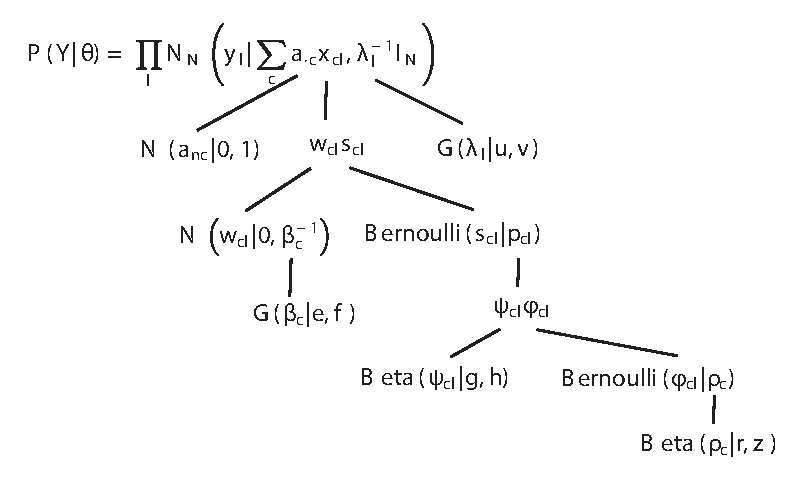
\includegraphics[width=\textwidth]{figures/singlecell/SDA.pdf}
	\caption[SDA]{
		\textbf{(A)} Schematic illustrating SDA
		\textbf{(B)} Density of gene loadings over all components with loadings separated into genes with PIPs > 0.5 (20\%) versus <0.5, indicating the sparsity of resulting gene loadings. PIP = Posterior Inclusion Probability that a gene loading is not equal to zero (i.e. not in the spike).
		\textbf{(C)} For each method, the fraction of all absolute gene loadings exceeding a ‘no loading’ sparsity threshold is shown, normalized by the maximum absolute loading across all components for that method. 
		\textbf{(D)} t-SNE projection of the cell scores from SDA. Each point it a cell, each coloured by their loading in component 5. Black arrow: the principle curve fit to the germ cell data, corresponding to the developmental ordering of each cell progressing through spermatogenesis. The coloured segmented line shows broad staging of spermatogenesis.
		\textbf{(E)} Gene loadings for component 5, plotted along the genome. Red genes: GWAS hits for human recombination rate.
		\textbf{(F)} Enrichment for GWAS hits of human recombination rate for all components. OR: Odds Ratio. P value by FET (main text). Positive (P) and negative (N) loadings are tested separately. For one-sided components (cell score range ratio >5) the minor side is omitted. Red horizontal line: p = 0.05 after Bonferroni correction for multiple testing.
	}
	\label{fig:SDA}
\end{figure}

We can perform the same dimensionality reduction on the \emph{transposed} cell scores or gene loadings to see how the components relate to each other rather than the cells (figure \ref{fig:tSNE_Components}). We find 7 major clusters of components and with hindsight these correspond to: 1) Spermatogonia, 2) Leptotene/Zygotene 3) Pachytene 4) Round Spermatid (Acrosomal) 5) Spermiogenesis 6) Somatic and 7) Somatic (Sertoli). We can see that our manual labelling of the components is consistent with the clusters.

\begin{figure}[H]
	\centering
	\includegraphics[width=\textwidth]{figures/singlecell/tSNE_Components.pdf}
	\caption[tSNE of Components]{A low dimensional representation of the components shows 7 clusters.}
	\label{fig:tSNE_Components}
\end{figure}

Visualisation of components through pseudotime shows that transcription during spermatogenesis can be represented as a series of overlapping components, each varying with different timescales (figure \ref{fig:SDA_overlapping}A\&B). Furthermore, these components are comprised of distinct gene sets enriched for distinct biological processes (figure \ref{fig:SDA_overlapping}C\&D).

\begin{figure}[H]
	\centering
	\includegraphics[width=\textwidth]{figures/singlecell/SDA_Overlaping.pdf}
	\caption[Overlapping SDA Components]{
		\textbf{(A)} For five example components, the cell scores for each cell are plotted through pseudotime, showing overlapping dynamic component activity. Component signs were chosen to be mainly positive (components have arbitrary sign). Color mappings as in panel B.
		\textbf{(B)} Stacked bar plot of cell component loadings for 14 germ components sorted by cell pseudotime. Each column corresponds to an individual cell and the total positive component loadings for each are normalized to one after flipping components to be mainly positive.
		\textbf{(C)} Shown are the top 10 gene loadings for each of the components in (B) represented as a heatmap. Most genes have strong loading on only one component.
		\textbf{(D)} Gene ontology enrichment analysis for biological processes in the top 250 genes for each component }
	\label{fig:SDA_overlapping}
\end{figure}



\section{Imputation}

In addition to identifying soft clusters and their marker genes, In the process of fitting the SDA model we have also effectively imputed the very sparse and noisy data. Multiplying out the cell scores and gene loadings matrix generates a matrix of the same dimensions as the original data but populated with the models predicted values. SDA imputation is able to estimate expression of individual genes even when in many cells zero reads are observed (figure \ref{fig:imputation}A). In addition SDA expression estimates have fewer outlying high values outside the genes main expression window. The destructive nature of the single cell RNAseq protocol means that it is not possible to determine the true expression vector for an individual cell. In order to determine if imputation is actually improving our estimates we use cross-validation. Specifically, we randomly assign each read to either a training or test set, predict gene expression based on the training set (using SDA, or another method for example the dedicated imputation method MAGIC from \cite{vanDijk2018Recovering}) and then evaluate our ability to rank gene expression using the test set (methods section \ref{sec:imputation_methods}). SDA imputation outperforms approaches using the raw data for essentially all cells in the test data (figure \ref{fig:imputation}B\&C).

While providing the most sparse representation (figure \ref{fig:SDA}C), SDA still imputes equally well, compared to other matrix factorizations and MAGIC \parencite{vanDijk2018Recovering} (figure\ref{fig:imputation}C \& \ref{fig:imputation_supp}A). Some cells gain more from imputation than others, the cells that gain the most are those with low library size (figure \ref{fig:imputation_supp}C).

Furthermore, by comparing the genes with the lowest correlation between NNMF and SDA imputed expression, we found that SDA provides additional biological insights for the same number of components (figure \ref{fig:imputation}D,E,F \& \ref{fig:imputation_supp}B). SDA infers multiple components for undifferentiated spermatogonia whereas NNMF only infers a single component resulting in imputed expression of \textit{Gfra1} and \textit{Lin28a} in the same cells (figure \ref{fig:imputation}D and figure \ref{fig:imputation_supp}B - no correlation for SDA component 50 \textit{Gfra1} Stem Cells). NNMF predicts a peak in the expression of X linked gene \textit{Rhox2h} even in WT cells, in which X chromosome activation due to Hormad1 KO does not occur, suggesting underfitting of the data with 50 components (figure \ref{fig:imputation}E). NNMF does not predict high expression of the adaptive immune cell marker \textit{Cd3g} (T-cell surface glycoprotein CD3 gamma chain), and when it predicts any expression it increases linearly with the innate immune cell marker \textit{Csf1r} (Macrophage Colony-Stimulating Factor 1 Receptor, or \textit{Cd115}) (figure \ref{fig:imputation}F). In contrast, SDA correctly predicts that \textit{Cd3g} and \textit{Csf1r} are not coexpressed in the same cells (see also figure \ref{fig:imputation_supp}B, no correlation for the SDA component 3 Lymphocytes).

In addition to obviating the need for further clustering and differential expression analyses, an advantage of using matrix factorization for imputation is the much smaller memory footprint required to store the results: on our dataset MAGIC data is 2.9 Gb whereas the SDA matrices are just 18 Mb (12.6 Mb when loadings with PIP <0.5 are set to 0).


\begin{figure}[H]
	\centering
	\includegraphics[width=\textwidth]{figures/singlecell/imputation&NNMF.pdf}
	\caption[SDA Imputation]{
		\textbf{(A)} For seven genes expressed at various stages of spermatogenesis unimputed normalised gene expression is shown alongside SDA imputed expression.
		\textbf{(B)} Prediction accuracy of seven predictors of gene expression trained on test data for an example individual cell. ‘Unimputed’ uses the training data directly, ‘Mean Cell’ uses the mean across all cells, matrix factorisation approaches SDA, PCA, ICA, NNMF, and a dedicated imputation approach, MAGIC.
		\textbf{(C)} Comparison of AUCs (Area under the curve) for all cells using various methods (same colour scheme as part B).
		\textbf{(D)} Zoomed versions of the t-SNE projection (with full t-SNE for context): cells are coloured by expression using a three channel ternary colour scheme with the amount of blue, green, red representing the respective expression levels of \textit{Lin28a}, \textit{Nanos1}, and \textit{Gfra1}.
		\textbf{(E)} Imputed expression of X chromosomal gene \textit{Rhox2h} from either the SDA or NNMF decomposition, split into cells we know to be either WT or \textit{Hormad1\textsuperscript{-/-}} genotype.
		\textbf{(F)} Imputed expression of \textit{Cd3g} and \textit{Csf1r} for both NNMF and SDA.}
	\label{fig:imputation}
\end{figure}

\begin{figure}[H]
	\centering
	\includegraphics[width=\textwidth]{figures/singlecell/Imputation_Supp.pdf}
	\caption[Imputation Supplement]{
		\textbf{(A)} Imputed expression of an example gene (\textit{Smok2b}) for different methods, to illustrate the similar predictions as shown in figure \ref{fig:imputation}B and \ref{fig:imputation}C.
		\textbf{(B)} Overall, NNMF infers similar components to SDA. The heatmap shows Pearson correlations between different pairs of gene loading vectors from SDA and NNMF (with procrustes rotation applied, methods section \ref{sec:imputation_methods}).
		\textbf{(C)} The fold improvement in AUC when comparing SDA imputation to the unimputed data, plotted as a function of cell library size.
	}
	\label{fig:imputation_supp}
\end{figure}

\section{Mutant Genotypes}

Given we combined both wild-type and mutant cells in our analysis it is important to check that the components representing wild type processes are not unduly affected by this mixing. In order to quantify the robustness of our conclusions to this decision to combine mutant and wild-type strains, we performed a separate SDA analysis using just wild-type cells (the ‘WT’ analysis) and compared the results.

Factor analyses naturally have a degree of unidentifiability, whereas in SDA the sparsity prior helps to make the model identifiable across different seeds. For different data however, the gene loadings matrix may be a rotated version in which components are linearly split or combined. A procrustean rotation can align two matrices (here gene loadings) onto an equivalent set of axes. Therefore, for fair comparison across SDA runs with different datasets, we compared the correlation of the gene loadings after procrustean rotation which tells us if the components inferred are effectively the same.

We found that most components generated from an SDA analysis of only wild-type data were also observed in the joint analysis of wild-type and mutant data. The most important WT components (those with high total cell score) have high correlations with components in the mixed SDA run (figure \ref{fig:WT_vs_Mixed}). Some components such as ``Mix38 X activation'' are not represented in the WT decomposition because they represent mutant-specific processes. Other components such as ``Mix44 Leptotene-Zygotene'' do not appear as these cells are numerous only in mutant samples which lack the more abundant later stages of cells.

By visualising the rotation matrix from the procrustean analysis we can see which components have been rotated. For example ``Mix17 spermiogenesis'' is a linear combination of WT component 46 and 7 (figure \ref{fig:WT_Mix_Rotation}). We can also visualise the correlations directly as in figure \ref{fig:WT_Mix_Correlation}.

\begin{figure}[H]
	\centering
	\includegraphics[width=\textwidth]{figures/singlecell/correlation_matrix_rotated.pdf}
	\caption[Wild Type vs Mixed SDA]{Here we show as a heatmap the pearson correlation of component gene loadings between a procrustean rotation of the WT gene loadings and the Mixed SDA gene loadings. The ‘sum abs cell score’ annotation shows the sum of the absolute cell scores for that component (larger number indicates a more important component). The ‘max cell score’ annotation indicates the maximum cell score for each component (a larger maximum indicates overfitting to a single/small number of cells).}
	\label{fig:WT_vs_Mixed}
\end{figure}

\begin{figure}[H]
	\centering
	\includegraphics[width=\textwidth]{figures/singlecell/rotation_matrix_sparseNEW.pdf}
	\caption[Procrustean Rotation Matrix]{This heatmap shows the procrustean rotation matrix (with absolute values < 0.35 rounded down to 0).}
	\label{fig:WT_Mix_Rotation}
\end{figure}

\begin{figure}[H]
	\centering
	\includegraphics[width=\textwidth]{figures/singlecell/UdifSpg_gene_scatterplot.pdf}
	\caption[Component 31 WT vs Mixed]{An example scatterplot comparing the gene loadings for one cognate SDA component (C31) between WT and Mixed SDA runs. The correlation is high.}
	\label{fig:WT_Mix_Correlation}
\end{figure}


\section{Non Meiotic Components}

Given we combined multiple experimental batches it's important to correct for batch effects and SDA provides a simple approach as some inferred components will capture these effects and can be removed.

Component 22 gene loadings are highly enriched in ribosomal proteins (50 of the top 100 loadings are non pseudogene ribosomal genes - of which there are 99, figure \ref{fig:NonMeiotic}A). However unlike ribosomal component 43, the cell scores for component 22 are associated with whether the sequencing was done on MiSeq or HiSeq Illumina machines and so this component is likely a batch effect (figure \ref{fig:NonMeiotic}B).

Component 12 has high cell loadings for \textit{Hormad1\textsuperscript{-/-}} cells, but these loadings are largely positive for the first two libraries, and negative for the last library (figure \ref{fig:NonMeiotic}C,D).

Component 9 contains 41 out of 57 of the respiratory complex I, III, and IV genes (complex II is an alternative pathway) (figure \ref{fig:NonMeiotic}E,F, $p = 7.4\times10^{-53}$, OR = 104 [95\% CI: 62.1,Inf] FET). It's not clear whether this component reflects real meiotic biology or potentially reflects cell stress induced by experimental processing (still a real biological process but not one that exists in vivo).

\begin{figure}[H]
	\centering
	\includegraphics[width=\textwidth]{figures/singlecell/NonMeiotic_Components.pdf}
	\caption[Non Meiotic Components]{
		\textbf{(A \& B)} Gene loadings and cell scores for component 22.
		\textbf{(C and D)} Gene loadings and cell scores for component 12.
		\textbf{(E)} Gene loadings for component 9. Genes that are (non-assembly) components of the electron transport chain proton pump genes are highlighted in red. This gene set is defined by the genes that match the regex ‘Uqc|Cox|Ndu’. Pseudogenes, and genes with ‘assembly|like’ in their name were excluded.
		\textbf{(F)} Enrichment of genes that are (non-assembly) components of the electron transport chain proton pump genes in the top 500 genes from each component.
	}
	\label{fig:NonMeiotic}
\end{figure}


\section{Components}

Assigning a cytologically defined stage to each component requires considerable manual work due to lack of any previous high resolution annotations. There are a number of issues that complicate assignment. Firstly as we have seen components activities are gradual and so there may be no well defined set of cells or start and end to a component. Components can be mixed sign (positive/negative), and one sign may be active in a different stage to the other. Stages themselves are not well defined in the literature with multiple definitions being used by different groups. Due to translational regulation the transcription of genes may not correspond to the detection of the protein, hence using commonly performed antibody based immunofluorescence can be misleading and so, if available, mRNA detection methods should be used for reference. Many studies only check protein expression, and often only by western blot from whole tissues to check testis specificity rather than spermatogenic stage. Even when mRNA is quantified developmentally the time points are often so widely spaced as to only permit vague conclusions about when expression starts. In addition, any literature references from human, or even rat, can have different expression patterns than mouse and so this evidence must be used with caution. Nonetheless, using a combination of evidence types from multiple genes for each component increases our confidence and precision enough such that we assigned each component to a stage(s) or cell type(s) most consistent with the available data.


\begin{figure}[H]
	\centering
	\includegraphics[width=\textwidth]{figures/singlecell/Cell_Scores.png}
	\caption[SDA Cell Scores]{Cell scores as coloured tSNE plots, excluding single cell components}
	\label{fig:Cell_Scores}
\end{figure}




\subsection{Telocytes}
Recently telocytes were found to be present in the mammalian (human) testis \parencite{Marini2018Reappraising, Kuroda2004Distribution}. We find one component (\#32) matching the known combination of markers for telocytes (\textit{Cd34} and \textit{Pdgfra} positive, \textit{Kit}, \textit{Pecam} and \textit{Acta2}/\textalpha-SMA negative). We also find many other genes are specific to this cluster (\textit{Dcn}, \textit{Col1a2}, \textit{Col1a2}, \textit{Col3a1}, \textit{Col6a1}, \textit{Col4a4}, \textit{Col4a1}, \textit{Col1a1}, \textit{Lamb1}, \textit{Lama2}, \textit{Lamb2}, \textit{Gsn}, \textit{Adamts5}, \textit{Mgp}), representing potential novel markers for this cell type in the testis. This component is highly enriched for the GO term ``extracellular matrix organization'' ($q = 4.3\times10^{-16}$, OR = 10.3). These cell's expression pattern matches what was described as an unknown mesenchymal cell population by \cite{Green2018Comprehensive} with expression of \textit{Tcf21}, \textit{Arx}, \textit{Vim}, and \textit{Col1A1}, but not \textit{Acta2} (\textalpha-SMA), or \textit{Cyp17a1}.


\subsection{Leydig Cells}
Component 40 broadly marks all Leydig cells and has high gene loadings for all the major genes required for testosterone production including \textit{Star}, \textit{Cyp11a1}, \textit{Hsd3b}, \textit{Cyp17a1}, and \textit{Hsd17b} (figure \ref{fig:MiscComponents}F, \cite{Stojkov2013Orally}) in addition to other markers of Leydig cells including \textit{Insl3} and \textit{Ptgds} \parencite{Balvers1998RelaxinLike, Baker2001Expression}. This component is most highly enriched for the GO term ``steroid metabolic process'' ($q = 5.3\times10^{-23}$, OR = 11.3)

Component 26 splits Leydig cells into two main groups, distinguished by the expression of \textit{Fabp3}, \textit{Gstm1}, \textit{Gsta3}, and \textit{Ass1}.

Component 24 is a subtype of the \textit{Fabp3} expressing C26 positive cells, which has high expression of \textit{Gstm3}, \textit{Mt3}, \textit{Thrsp}, and \textit{Jak3}, but also a number of pseudogene versions of genes that are normally expressed leydig genes: \textit{Gstm2-ps1}, \textit{Gm6665} (another \textit{Gstm2} pseudogene), \textit{Fabp3-ps1}, \textit{Gm8834} (\textit{Gstm3} pseudogene), \textit{Gm5096} (\textit{Bhmt} pseudogene), \textit{Gm6977} (\textit{Fth1} pseudogene), \textit{Gm7049} (\textit{Me1} pseudogene).

Component 19 marks cells in both major groups and is distinguished by high expression of a group endopeptidases encoded in a 300kb locus on chromosome 7 including \textit{Klk1}, \textit{Klk1b1}, \textit{Klk1b21}, \textit{Klk1b22}, \textit{Klk1b24} and \textit{Klk1b27}. Some of these genes are known to be specifically expressed in Leydig cells and may be involved in remodelling of the extracellular matrix \parencite{Sanz2013RiboTag, Matsui2000Cloning, Matsui2001Mouse, Matsui2005Characterization}.

\subsection{Sertoli Cells}

Component 37 is active in cells expressing \textit{Wipf3} (aka CR16) and \textit{Ncoa2} (aka TIF2) both of which are required for fertility and have Sertoli restricted expression \parencite{Suetsugu2007Malespecific, Gehin2002Function}). In addition \textit{Nxf3} is specifically expressed in Sertoli cells but not required for spermatogenesis \parencite{Zhou2011Nxf3}.

Component 45 is also likely to be active in Sertoli cells, but merges with the pachytene cells, very speculatively representing phagocytosis of apoptosing cells.

%16

\subsection{Macrophages}
We find one component (\#11) representing macrophage cells. This component has high loadings for \textit{Csf1r} (macrophage colony-stimulating factor receptor, aka CD115), \textit{Cd163} (macrophage scavenger receptor), \textit{Cd68}, \textit{Adgre1} (aka F4/80), \textit{Itgam} (aka CD11b), \textit{Mrc1}, \textit{Cx3cr1}, \textit{Fcgr3}, and the complement genes \textit{C1qa}, \textit{C1qb}, and \textit{C1qc} \parencite{Mossadegh-Keller2017Developmental, Fabriek2005macrophage, Sasmono2012Generation}. Macrophages are professional antigen-presenting cells and the highest enriched GO term for this component is ``antigen processing and presentation of peptide antigen'' ($q = 1.4\times10^{-19}$, OR = 9.5) driven by genes including the MHC I and II genes \textit{H2-D1}, \textit{H2-Aa}, \textit{H2-Ab1}, \textit{H2-Eb1}, \textit{H2-K1}, \textit{H2-DMa}, \textit{H2-T23)}, \textit{B2m}, and the other immune related genes such as \textit{Cd74}, \textit{Fcgr3}, \textit{Fcgr2b}, \textit{Fcer1g}.

Immunohistochemical staining of ADGRE1 in \textit{Hormad\textsuperscript{-/-}} and \textit{Mlh3\textsuperscript{-/-}} but not wild type mice found that macrophages were present within the tubule, which is typically regarded as immune privileged partly due to the blood-testis barrier formed by Sertoli cell tight junctions \parencite{Fijak2006testis}. Macrophages have previously been reported within the adluminal compartment, although always in the context of testicular defects \parencite{Frungieri2002Number, Goluza2014Macrophages}. Intriguingly component 11 is also specifically and strongly enriched for GWAS hits for Alzheimer's ($p = 1.3\times10^{-11}$, OR = 65.9 by FET, figure \ref{fig:MiscComponents}E) and these cells are also marked by the Alzheimer's gene \textit{Apoe} in in \textit{Mlh3\textsuperscript{-/-}} (25/707 tubules, 3.5\%, $p<2.2\times10^{-16}$) and \textit{Hormad\textsuperscript{-/-}} (98/1756 tubules, 5.6\%, $p<2.2\times10^{-16}$) but not wild type tubules (0/2496 tubules). Co-staining of ADGRE1 with an antibody for activated CASPASE-3, a marker of apoptosis, failed to identify any double positive cells, excluding the possibility that intratubular ADGRE1 protein expression was somehow an artifact of an apoptotic cell population. The mechanisms by which macrophages transit the blood-testis barrier, and the corresponding cues for migration, await further investigation.


\subsection{Lymphocytes}
Component 3 is highly enriched for genes involved in T cell activation ($q = 1.4\times10^{-19}$, OR = 7.6) and has high loadings for (T-cell) lymphocyte genes including \textit{Ptprc} (aka CD45, leukocyte common antigen), \textit{Cd2} (aka T-cell surface antigen) \parencite{Murray2011Protective, Murphy2012Janeway}, \textit{Ms4a4b} (high protein expression in T and NK but not B cells - \cite{Xu2010MS4a4B}), and the CD3 T-cell receptor complex genes: \textit{Cd3g}, \textit{Cd3d}, \textit{Cd3e}, \textit{Trbc2}, \textit{Trac} \parencite{Call2002Organizing}.


\subsection{Peritubular Myoid}
% 21??

Component 10 is active in a small number of cells, likely to be peritubular myoid cells due to co-expression of \textit{Cnn3}, \textit{Edn1} (Endothelin), \textit{Myh11} (Smooth muscle myosin heavy chain), and \textit{Acta2} (Smooth muscle actin) \parencite{Mayerhofer2013Human}. The most significant GO term is ``muscle tissue development'' ($q = 8.8\times10^{-8}$, OR = 4.97).


\subsection{Spermatogonia}

% Spermatogonia can are the most undifferentiated germ cells in the adult body. There are a number of different types which can be categorised according to the Oakberg scheme in mice \parencite{Oakberg1971Spermatogonial}. As are the most stem cell like, which divide into Apr, Aal4, Aal be \parencite{vanPelt1990Synchronization}

Five components correspond to processes in spermatogonia. Component 31 represents undifferentiated spermatogonia expressing \textit{Zbtb16} (aka \textit{Plzf}) \parencite{Buaas2004Plzf} and \textit{Foxo1} \parencite{Goertz2011Foxo1}, while component 50 splits these cells into two subpopulations, the first expressing \textit{Glis3} \parencite{Kang2016Transcription} and \textit{Gfra1} - shown to be expressed in a subset of $A_s$ and required for $A_s$ self renewal by acting as a co-receptor for GNDF \parencite{Meng2000Regulation,He2007Gfra1}. The second subpopulation expresses \textit{Nanos3} \parencite{Suzuki2009heterogeneity}, \textit{Lin28a} \parencite{Zheng2009pluripotency} and \textit{Foxf1}. Component 7 likely represents $A_{1-4}$ spermatogonia as they express c-Kit which is expressed in differentiated (not undifferentiated) spermatogonia \parencite{Manova1990Gonadal,Schrans-Stassen1999Differential} and is required for the A1 to Al divisions \parencite{Yoshinaga1991Role}. These cells also express \textit{Stra8} which is expressed from type A spermatogonia through to preleptotene cells in response to retinoic acid \parencite{Oulad-Abdelghani1996Characterization,Zhou2008Expression,Endo2015Periodic} and is required for premeiotic DNA replication \parencite{Baltus2006germ}. We find they these cells are also well marked by \textit{Plppr3}, \textit{Sertad4}, \textit{Met}, \textit{Jade2}, \textit{Nanos1}, \textit{Glis1} and \textit{Glis2}. Component 2 includes \textit{Ctcfl}, \textit{Pou4f1}, and \textit{Esx1} - likely representing intermediate and type B spermatogonia \parencite{Sleutels2012male, Budhram-Mahadeo2001closely, Maezawa2018Dynamic, Li1997Esx1, Branford1997Spx1}. Component 33 is broad component covering all the stages of spermatogonia.


\subsection{\label{sec:leptotene}(pre)Leptotene \& Zygotene}
Component 5 includes many genes required for the creation and repair of meiotic double strand breaks. This includes \textit{Prdm9} itself; components of the meiotic cohesin complex \textit{Rad21l}, \textit{Smc1b}, \textit{Smc3}, \textit{Stag3} and \textit{Esco2} \parencite{Rankin2015Complex}; components of the telomere tethering complex \textit{Terb1}, \textit{Terb2}, \textit{Spdya}, and \textit{Sun1} \parencite{Ding2007SUN1, Tu2017Speedy, Wang2019meiotic}; genes involved in creating DSBs \textit{Mei1}, \textit{Ccdc36} (\textit{Iho1}), \textit{Spo11} partner \textit{Top6bl} (\textit{Gm960}), and regulator \textit{Atm} \parencite{Lukaszewicz2018Control, Reinholdt2005Mei1, Robert2016TopoVIBLike, Stanzione2016Meiotic, Vrielynck2016DNA}; proteins required for the creation and processing of the ssDNA intermediates and their regulators: \textit{Mcm8}, \textit{Dmc1}, \textit{Rad51}, \textit{Rad51ap2}, \textit{Atr}, \textit{Brca2}, \textit{Tex15}, \textit{Meilb2} (\textit{Hsf2bp}), \textit{Meiob}, and \textit{Spata22} \parencite{Brown2015Small, Brown2014DNA, Dai2017Meiotic, Kovalenko2006RAD51AP2, Lee2015MCM89, Martinez2016BRCA2, Pacheco2018ATR, Ribeiro2018MEIOB, Widger2018ATR, Xu2017Meiosisspecific, Yang2008Mouse, Zhang2019meiosisspecific}; class I crossover (ZMM group) proteins \textit{Shoc1} (\textit{Zip2} orthologue), \textit{Tex11} (\textit{Zip4} orthologue), \textit{Msh5}, \textit{Hfm1} (\textit{Mer3} orthologue) and regulator \textit{Brip1} (\textit{FancJ}) \parencite{Adelman2008ZIP4H, Guiraldelli2018SHOC1, Guiraldelli2013Mouse, Rakshambikai2013Structural, Sun2016FancJ}; as well as components of the synaptonemal complex \textit{Sycp1}, \textit{Sycp2}, \textit{Sycp3}, \textit{Syce2}, \textit{Syce3}, \textit{Tex12}, and \textit{Six6os1} (\textit{4930447C04Rik}) \parencite{Gomez-H2016C14ORF39, Syrjanen2014molecular}.


This component is also highly enriched for GWAS hits of recombination rate in Icelandic humans \parencite{Halldorsson2019Characterizing}. Of the 24 significant GWAS loci identified with confidently associated causal genes, more than half (13) rank within the top 300 genes of this component, and almost all (20) rank within the top 1300 genes ($p = 5.2\times10^{-18}$, OR = 77.8 [95\% CI:36.4,Inf] and $p = 2.4\times10^{-20}$, OR = 70.1 [95\% CI:26.9,Inf] respectively by fisher's exact test [FET]). One of the hits, \textit{Msh4}, is not ranked highly in this component (2734th out of 19262), however, it is known to function as a heterodimer with \textit{Msh5}, which ranks 34th \parencite{Rakshambikai2013Structural}. This highlights one of the advantages of single cell RNAseq compared to GWAS for target discovery in that it does not rely on the presence of (perhaps rare, small effect) genetic variants. In addition it directly provides a list of genes rather than SNPs affecting unknown causal genes, For example the previous GWAS had identified a SNP in the intron of \textit{Ccdc43}, however our expression data strongly suggested the adjacent gene \textit{Meioc} (aka \textit{C17orf104}) as the causal gene (ranked 183rd vs 13,651st in component 5) in addition to the subsequent reports that \textit{Meioc} is responsible for maintaining an extended meiotic prophase \parencite{Abby2016Implementation, Kong2014Common, Soh2017Meioc}. 

The strong enrichment of genes involved in recombination in this component suggests other highly ranked genes of unknown function could also play key roles in this process. This proved to be the case for two such genes during the preparation of this manuscript. Firstly \textit{Ankrd31} (ranked 102nd) was found to control the number, timing, and location of double strand breaks in meiosis \parencite{Boekhout2018REC114, Papanikos2018ANKRD31} and \textit{Hsf2bp} (now \textit{Meilb2}, ranked 194th) was found to be a master regulator of meiotic recombinases \parencite{Zhang2019meiosisspecific}. One candidate, \textit{Zcwpw1}, will be the subject of chapter \ref{ch:3-Zcw}.


\subsection{Pachytene}

Pachytene is the longest stage of prophase I (\textasciitilde7 days in mice) and has the highest non-ribosomal RNA synthesis activity \parencite{Monesi1978Chapter}. Accordingly, a number of components represent this stage and have many highly loading genes.

Many of the proteins expressed at this stage are stored for later use when transcription is repressed due to nuclear condensation. Y-box proteins are abundant in spermatocytes where they bind to and repress translation of mRNA \parencite[reviewed in][]{Kleene2016Positiondependent}. \textit{Ybx2} (aka \textit{Mys2}) has a high loading in component 42 (rank 223), which was found translated from pachytene onwards \parencite{Kwon1993Proteins, Oko1996Germ} (transcribed from day 17 \& in pachytene cells \parencite{Gu1998Mammalian}) and is required for fertility \parencite{Yang2005Absence}. \textit{Ybx1} (\textit{Msy1}, rank 5) with reported mRNA detectable by northern blot from day 15 (pachytene) \parencite{Tafuri1993mouse}. \textit{Ybx3} (aka \textit{Msy4}, rank 28), also has a high loading and is detected as protein in mid-pachytene cells \parencite{Davies2000SequenceSpecific} and extended expression causes infertility \parencite{Giorgini2002Translational}

Poly(A) binding proteins also bind to and regulate mRNA \parencite[reviewed in][]{Ozturk2018Potential}. \textit{Pabpc1} and \textit{Pabpc2} both have high loadings in component 42 (rank 4 and 52) and are detectable from pachytene onwards \parencite{C.Kleene1994Developmental, Gu1995Poly, Kleene1998Mouse, Lee2000Expression, Kimura2009Characterization}. \textit{Pabpc6} also has a high loading (rank 22) but is understudied in comparison.

Spermatocytes have specialist energetic requirements and many core enzymes have different isoforms in spermatocytes. Testis specific lactate dehydrogenase \textit{Ldhc} is ranked highly (1st) in component 42 \parencite{Goldberg1963Lactic, Blanco1963Lactate, Goldberg2010LDHC}, in addition to \textit{Ldha} (rank 83) and \textit{Ldhal6b} (rank 19) \parencite{Wang2005Cloning}, and another glycolytic enzyme \textit{Pgam2} (rank 107) for which protein expression was found from pachytene onwards \parencite{Fundele1987Developmental}.

The earliest pachytene component (\#13) has a number of highly loading piwi associated genes: \textit{Piwil1} (Miwi), \textit{Tdrd1} (Tudor), \textit{Tdrd5} (Tejas), \textit{Pld6} (Zucchini), and \textit{Piwil2} (Mili) (rank 4, 7, 8, 42, 84). Other pachytene components also have high loading piwi associated genes such as \textit{Ddx4} (Mvh/Basa) and \textit{Tdrd9} (SpnE) in component \#47 (rank 9 and 32), and \textit{Mael} (Maelstrom) in component \#39 (rank 42). While the piwi pathway is most commonly associated with transposon silencing, in male germ cells there is a second phase of activity during pachytene where piRNAs originate from piRNA clusters rather than transposable elements, and have been proposed to direct transcriptional silencing of mRNAs \parencite{Gou2014Pachytene, Iwasaki2015PIWIInteracting}. Component \#39 also has high loadings for many subunits of the chaperonin complex which enables proper folding of actin and tubulin \parencite{Dun2012role} (\textit{Tcp1}, \textit{Cct7}, \textit{Cct4}, \textit{Cct3}, \textit{Cct6a}, \textit{Cct5}, rank 23, 117, 124, 212, 325, 333). Most of these genes are most highly expressed in the testis compared to other tissues in GTEx.

Pachytene components can be readily identified by the relative lack of loadings on the X and Y chromosomes (figure \ref{fig:MSCI}D,E). This is due to a process where homologous chromosomes that fail to synapse are marked by HORMAD1, HORMAD2 and BRCA1. This is followed by recruitment of ATR and the creation of $\gamma$H2AX resulting in transcriptional silencing (Meiotic Silencing of Unsynapsed Chromatin). As the X and Y chromosomes are only partially homologous they fail to fully synapse and are silenced by this processes (Meiotic Sex Chromosome Inactivation, MSCI) \parencite{Turner2007Meiotic, Turner2015Meiotic}.

Pseudotime analysis provides quantitative, high-resolution insights into MSCI. We are able to track this process through pseudotime by visualising the ratio of sex to autosomal expression through pseudotime (figure \ref{fig:MSCI}A \& \ref{fig:MSCI_supp}A). The ratio drops sharply (possibly exaggerated by inefficient cell capture) to almost 0 before gradually recovering, although to a level below that of the original starting ratio. It has previously been reported that some sex chromosome genes are able to escape MSCI \parencite{daCruz2016Transcriptome, Soumillon2013Cellular}. However, we were unable to detect expression of these genes during the time at which MSCI is active (figure \ref{fig:MSCI}C \& \ref{fig:MSCI_supp}B). Many of the genes had high expression just before or after MSCI, suggesting that they were previously identified due to the low stage-resolution of the previous study. 

\begin{figure}[H]
	\centering
	\includegraphics[width=\textwidth]{figures/singlecell/MSCI.pdf}
	\caption[Meiotic Sex Chromosome Inactivation]{
		\textbf{(A)} The sum of imputed expression for all genes on the X chromosome divided by that of the autosomes (y-axis).
		\textbf{(B)} We do not observe that haploid cells obviously split into two populations due to lack of sex chromosome transcript sharing, in part A. Here were simulate what we might expect to see if there was indeed a lack of sharing (methods section \ref{sec:msci_methods}).
		\textbf{(C)} Smoothed expression values (unimputed, adaptive GAM smoothing with formula ``y \textasciitilde s(x, bs = ad)'') are shown for each gene reported to escape MSCI \parencite{daCruz2016Transcriptome} excepting \textit{H2al1e}, \textit{H2al1c}, and \textit{Gm10096} which were below our dataset's expression detection threshold.
		\textbf{(D)} Component 42 (Pachytene) cell scores in t-SNE space.
		\textbf{(E)} Component 42 gene loadings. This component represents genes active during the pachytene stage of meiosis; note the striking lack of sex chromosome gene loadings, due to MSCI.
	}
	\label{fig:MSCI}
\end{figure}

\begin{figure}[H]
	\centering
	\includegraphics[width=\textwidth]{figures/singlecell/MSCI_supp.pdf}
	\caption[MSCI Supplement]{
		\textbf{(A)} As for Figure \ref{fig:MSCI}A, but Y chromosome instead of X. Due to lower number of expressed genes on the Y chromosome MSCI is not as clear and individual genes can influence the overall ratio to a large degree.
		\textbf{(B)} As for Figure \ref{fig:MSCI}C, but each gene is shown individually.}
	\label{fig:MSCI_supp}
\end{figure}


In addition to MSCI, we might expect to observe a lack of sex chromosome transcripts due to the lack of either an X or Y chromosome in the haploid cells post meiotic division. However, from the mitotic divisions of the spermatogonia onwards cytokinesis does not fully complete and $\mu$m-wide cytoplasmic bridges are formed between adjacent cells such that the cytoplasm could be shared across a syncytium of cells \parencite{Greenbaum2011Germ}. Whilst theoretically thousands of cells could be connected in practise up to 650 connected cells have been observed \parencite{Ren1991Clonal}. The extent to which mRNA sharing occurs is unknown although efficient sharing has been shown for individual genes \parencite{Braun1989Genetically}. If many genes were not shared we would expect to see two populations of cells after the meiotic divisions with high and low X chromosome expression respectively. However, we observe a marginal distribution of X expression conditional on pseudotime that is unimodal - suggesting that mRNA (on the X chromosome at least) is efficiently shared (figure \ref{fig:MSCI}B).

There remains a possibility that some individual or group of genes are not shared, such as has been observed for autosomal genes in a mutant heterozygous context: the t-complex responder mutant (\textit{Smok\textsuperscript{Tcr}}) which functions as an antidote in the poison-antidote meiotic drive system of the t-complex \parencite{Herrmann1999protein, Veron2009Retention} and \textit{Spam1} which causes transmission ratio distortion in Robertsonian (Rb) translocation-bearing mice \parencite{Martin-DeLeon2005Spam1associated}. Indeed a recent report using hybrid mice claimed widespread haploid biased gene expression \parencite{Bhutani2019Widespread}.


\subsection{Hormad1 Sex Chromosome Activation}
In addition to the pachytene components with lack of loadings on the sex chromosome we also find a component (\#38) with an \textit{excess} of sex chromosome loadings relative to the autosomes (figure \ref{fig:Hormad1}A). This component is active exclusively in a subset of \textit{Hormad1\textsuperscript{-/-}} cells that diverge from the normal pseudotime around Zygotene stage \ref{fig:MiscComponents}C. Note that as \textit{Hormad1\textsuperscript{-/-}} mice arrest at early Pachytene, once the cells diverge the pseudotimes can no longer be compared to the wild type pachytene cells and are perhaps considerably compressed due to the almost perpendicular direction in tSNE space \parencite{Shin2010Hormad1}. HORMAD1 marks unsynapsed chromosomes, so when HORAMD1 is absent (as in the KO) it appears as though the sex chromosomes are fully synapsed and transcriptional silencing fails to occur. We find that not only does \textit{Hormad1\textsuperscript{-/-}} fail to silence previously expressed sex-linked genes, many previously \textit{unexpressed} sex-linked genes such as \textit{Rhox2h} have high expression (figure \ref{fig:Hormad1}B). Interestingly, there are also multiple autosomal genes with high loadings. This may be due to ectopic expression of sex-linked transcription factors; for example, \textit{Zfy1} and \textit{Zfy2} were previously shown to cause pachytene arrest when forcibly expressed \parencite{Royo2010Evidence}. We find a very strong association between genes in this component and genes overexpressed in mice which have mutations in either \textit{Hormad1} ($p = 2.2\times10^{-39}$ OR = 184) or \textit{Trip13} which is required for HORMAD1 removal from synapsed chromosomes ($p = 1.3\times10^{-157}$ OR = 115) \parencite{Ortega2016Surveillance, Wojtasz2009Mouse} (figure \ref{fig:MiscComponents}A,B).

\begin{figure}[H]
	\centering
	\includegraphics[width=\textwidth]{figures/singlecell/Hormad1_two.pdf}
	\caption[Hormad1 KO Component]{
		\textbf{(A)} Gene loadings for component \#39 shown along the genome.
		\textbf{(B)} Gene expression for high loadings genes from chromosome 1 (\textit{A830018L16Rik}) and X (\textit{Rhox2h}).
	}
	\label{fig:Hormad1}
\end{figure}


\begin{figure}[H]
	\centering
	\includegraphics[width=\textwidth]{figures/singlecell/Fig4_S3.pdf}
	\caption[Misc. Components]{
		\textbf{(A)} Enrichment of component 38 gene loadings for genes previously identified as overexpressed in both \textit{Trip13\textsuperscript{-/-}} and \textit{Hormad1\textsuperscript{-/-}} mutants. Component 38 (X Activation) gene loadings are shown ordered by rank (high-to-low) with the genes previously identified as overexpressed in \textit{Hormad1\textsuperscript{-/-}} and \textit{Trip13\textsuperscript{-/-}} mice highlighted as rug plots.
		\textbf{(B)} Fisher’s test was used to test for enrichment of genes previously identified as overexpressed in \textit{Hormad1\textsuperscript{-/-}} and \textit{Trip13\textsuperscript{-/-}} mice in the top 500 genes of each component. Positive and negative loadings for each component are analysed separately; thus 38N is the negative gene loadings for component 38 and 38P the positive ones. The positive loadings of component 38 are highly and specifically enriched for these genes. Component enrichments are further coloured red and blue to indicate the primary cell type with loading on each component (red = germ cell, blue = somatic cell). 
		\textbf{(C)} Cell scores for component 38 in t-SNE space. The cells with component 38 active are localized to a group of cells which diverge from the pseudotime-line just before pachytene.
		\textbf{(D)} MSCI in t-SNE space. The cells with active component 38 also have a high ratio of sex to autosome expression ratio, showing that not only do these cells fail to silence sex linked genes but they are actively overexpressed.
		\textbf{(E)} Gene loadings and cell scores for component 11 (Macrophages). Genes with GWAS signals for Alzheimer's disease are highlighted in red. 
		\textbf{(F)} Gene loadings for component 40 (Leydig cells), with key genes of testosterone synthesis highlighted in red. The pathway of testosterone synthesis is shown with genes that have high loadings in component 40 highlighted (Adapted from \cite{Stojkov2013Orally}).
	}
	\label{fig:MiscComponents}
\end{figure}

\subsection{Cul4a, Mlh3, and Cnp Mutants}
CUL4A is a major component of the E3 ubiquitin ligase complex called CRL4 which is known to regulate cell cycle, DNA replication, DNA repair, and chromatin remodelling \parencite{Dubiel2018Cullin}. Studies on \textit{Cul4a\textsuperscript{-/-}} mice noted that some spermatocytes arrest at the pachytene stage of meiosis I induced by the pachytene checkpoint, whereas remaining spermatocytes complete meiosis but the resulting spermatozoa present oligoasthenospermia and severe malformations \parencite{Yin2011E3}. The molecular basis of the observed abnormal phenotypes in spermatozoa remains unclear. We identified a single SDA component (\#25) that was highly specific to \textit{Cul4a\textsuperscript{-/-}} cells. This component corresponds to dozens of genes that are overexpressed in \textit{Cul4a\textsuperscript{-/-}} mutants when compared to all other strains, with GO enrichments related to spermatid development, motility and capacitation. These findings are consistent with the observed phenotype of \textit{Cul4a\textsuperscript{-/-}} mice and provide new leads to investigate mechanisms of pathology.

MLH3 is an essential protein required for crossover formation in early meiosis and for binding of MLH1 to meiotic chromosomes. Studies on \textit{Mlh3\textsuperscript{-/-}} testes have shown depletion of spermatocytes and some spermatogonia due to apoptosis in diplonema induced by a reduction of chiasmata and a loss of recombination nodules \parencite{Lipkin2002Meiotic}. Interestingly, in contrast to \textit{Hormad1\textsuperscript{-/-}}, we found no obvious transcriptional phenotype in \textit{Mlh3\textsuperscript{-/-}} cells either by SDA analysis or by comparison of expression levels between hard-clustered wild-type and mutant cells (other than differential expression of \textit{Mlh3}). Instead, \textit{Mlh3\textsuperscript{-/-}} spermatocytes might simply trigger apoptosis through existing checkpoint protein machinery assembled earlier in development (figure \ref{fig:tsneGroups}).

Similarly, the cells from \textit{Cnp} mutant mice did not form distinct clusters, nor did they show SDA component loadings distinct from wild-type cells. Although the presence of multinucleated giant cells, hypocellular seminiferous tubules and infertile phenotype in these mice point to a serious defect in spermatogenesis, it is difficult to determine which stages are affected using single-cell expression data. One possible explanation of missing important biological signals may be that \textit{Cnp} mice present a partial arrest phenotype which masks the developmental abnormalities. Another possible explanation is that droplet-based sequencing library preparation may under sample the cells with aberrant transcriptional signatures, for example due to failure of oil droplets to encapsulate the giant cells.

\begin{figure}[H]
	\centering
	\includegraphics[width=\textwidth]{figures/singlecell/tsne_groups.pdf}
	\caption[Experimental groups in tSNE space]{
		Cells are shown projected by tSNE into two dimensions, with cells coloured by genotype or stage as separated by FACS (SPG: Spermatogonia, SPCI: Primary Spermatocytes, SPCII: Secondary Spermatocytes, SPD: Spermatids).
	}
	\label{fig:tsneGroups}
\end{figure}



\subsection{Meiotic Divisions}
Component 20 contains high loadings for cell cycle associated genes such as the cyclin \textit{Ccna1} (rank 45) which is expressed from late pachytene through until just after the meiotic divisions \parencite{Sweeney1996distinct} for which it is required \parencite{Liu1998Cyclin}. The cyclin \textit{Ccnb1} controlling the G2/M transition is also present (rank 8), along with its activators \textit{Aurka}, \textit{Bora}, \textit{Plk1}, and \textit{Cdc25a} (ranks 33, 83, 65, and 75) \parencite[reviewed in][]{Joukov2018AuroraPLK1}. The CDK2 inhibitor \textit{Cdkn3} (aka KAP1, \parencite{Poon1995Dephosphorylation}), \textit{Rgcc} (regulator of cell cyle) which is required for G2/M transition \parencite{Saigusa2007RGC32}, anaphase promoting complex activator and \textit{Cdc20} homologue \textit{Fzr1} \parencite{Holt2014APC}, and Mitotic Checkpoint Complex antagonist \textit{Mad2l1bp} (\textit{p31comet}) \parencite{Habu2002Identification} also have highly ranked loadings in component 20 (ranks 4, 35, 90, and 118). In addition, the positive and negative loadings are marginally significantly enriched for ``spindle checkpoint'' and ``chromosome segregation'' GO terms respectively (q = 0.029 \& 0.015, OR = 10.4 \& 3.7).

This component is also highly enriched for a family of proteins with a domain of unknown function (DUF622): \textit{1700001F09Rik}, \textit{Gm3453}, \textit{Gm10354}, \textit{Gm3149}, \textit{Gm8362}, \textit{Gm3127}, \textit{Gm17019}, \textit{Gm4181}, \textit{Speer4e}, \textit{Speer4b}, \textit{Gm9758}, \textit{Gm8232}, \textit{BC061237}, \textit{Gm5458}, \textit{4930572O03Rik}, \textit{Gm5800}, \textit{Gm7361}, \textit{Gm8220} (18 out of the top 88 genes). This family of genes is rodent specific and arose from duplication of the \textit{Dlg5} gene \parencite{Church2009Lineagespecific}. Interestingly it was reported that genes of this family have similar epigenetic profiles to that of the sex chromosomes in spermatogenesis \parencite{Moretti2016Expression}. This component is also host to a second family of ampliconic genes (Ssx - Synovial Sarcoma associated, on the X chromosome), discussed in further detail in section \ref{sec:ssx}.

\subsection{Round Spermatid}
Round spermatid component 30 contains many genes associated with the acrosome, an organelle which forms a nuclear cap containing hydrolytic enzymes used in fertilization \parencite{Ito2016Acrosome}. This component is highly enriched for ``cell wall macromolecule catabolic process'' by GO analysis  ($q = 1.47\times10^{-10}$, OR = 51.6), driven by a family of Chicken-type lysozyme genes: \textit{Spaca1}, \textit{Lyzl6}, \textit{Spaca3} (aka \textit{Lyzl3}), \textit{Lyzl1}, \textit{Lyzl4}, \textit{Spaca7}, \textit{Spaca4}, and \textit{1700016D06Rik} (rank 2, 10, 14, 16, 52, 58, 64, and 92).

SPACA1 (SAMP32) is first detected as protein in mice testis at stage 2 of round spermatids and is required for normal acrosome formation (globozoospermia) \parencite{Hao2002SAMP32,Fujihara2012SPACA1deficient}. LYZL6 was detected in primary and round spermatocytes in addition to the post-acrosomal area of spermatozoa \parencite{Wei2013Characterisation}.
 
SPACA3 (\textit{Lyzl3}, \textit{SLLP1}) was detected by gold particle immunostaining to be present at least in the acrosome of human sperm \parencite{Mandal2003SLLP1}, and the anterior acrosome and equatorial segment in mice caudal spermatozoa \parencite{Herrero2005Mouse}. Antibodies against SPACA3 prevented sperm egg binding suggesting a role for this protein in fertilisation \parencite{Herrero2005Mouse}.

LYZL1 was detected in the acrosomal matrix of mouse sperm by mass spectrometry, along with LYZL4, LYZL5, SPACA3 and SPACA5 \parencite{Guyonnet2012Isolation}. LYZL4 was detected in mouse spermatozoa in the acrosomal region \parencite{Sun2011Lyzl4}. In situ hybridisation analysis did not detect LYZL4 in human seminiferous tubules but instead in the epithelium of the epididymis \parencite{Zhang2005Molecular}. Lyzl4os (opposite strand antisense lncRNA) ranks 242nd.

SPACA7 expression substantially increases post meiotic divisions as measured by immunofluorescence, and can be detected in the acrosome by Immunogold electron microscopy \parencite{Korfanty2012Identification,Nguyen2014SPACA7}. SPACA4 (SAMP14) showed immunofluorescent staining restricted to the acrosomal region in washed human spermatozoa \parencite{Shetty2003SAMP14}. 1700016D06Rik (aka GC14) contains a Spaca7 domain and was previously reported as expressed in pachytene spermatocytes in contrast with our results \parencite{Anway2003Expression}. Other acrosomal genes not covered by the GO term include Lyzl5, Fam170b, Acrv1 (Spaca2), and Spata31 (AEP1) (rank 320, 56, 4, and 30).

Lyzl5 (Spaca5) is an X linked gene not previously studied apart from being detected by mass spectrometry as mentioned above \parencite{Guyonnet2012Isolation}. Fam170b which showed enrichment in the acrosome of round spermatids by immunohistochemistry and immunoflouresence \parencite{Li2015FAM170B}. Acrv1 (Spaca2) is highly specific to the acrosome as assessed by Immunohistochemistry \parencite{Osuru2014acrosomal}. Spata31 (aka AEP1 - Acrosome Expressed Protein) mRNA was detected by in situ hybridisation from postnatal 25 dpp (round spermatids) in rat \parencite{Luk2006Acrosomespecific}.
 
Another enriched GO term is ``fusion of sperm to egg plasma membrane involved in single fertilization'' ($q = 2.1\times10^{-6}$, OR = 32.2) driven by \textit{Spata46}, \textit{Lyzl6}, \textit{Spam1}, \textit{Eqtn}, \textit{Hyal5}, \textit{Izumo1} (rank 5, 10, 40, 73, 155 and 201).

\textit{Spata46} was detected in elongating spermatids and knock out resulted in abnormal sperm head shape and failure of sperm-egg fusion \parencite{Chen2016Deficiency}. \textit{Spam1} (Sperm Adhesion Molecule 1, aka PH-20 aka Hyal1) is a hyaluronidase originally discovered on guinea pig sperm heads \parencite{Myles1981Surface}, and later as required for binding to the egg \parencite{Primakoff1985role} and conserved among mammals \parencite{Lathrop1990cDNA} but is not required for fertilisation in mice \parencite{Baba2002Mouse}. Another hyaluronidase, \textit{Hyal5}, is also highly ranked in this component and potentially involved in penetration of mouse sperm \parencite{Kim2005Identification, Kimura2009Functional}. \textit{Eqtn} (Acrosome Formation-Associated Factor), is abundantly expressed in round spermatids and is required for the acrosomal reaction \parencite{Li2006Afaf, Hao2014Equatorin}.

\textit{Izumo1} and \textit{Izumo2} (rank 201 \& 589) are required for sperm to fuse with eggs by binding to the Juno receptor on the egg \parencite{Inoue2005immunoglobulin, Bianchi2014Juno}. \textit{Tmem190} (rank 50) was found to co-localise with IZUMO1 \parencite{Nishimura2011Characterization} and \textit{Glipr1l1} (rank 86) was found to form a complex with IZUMO1 and is required for optimal fertilisation \parencite{Gibbs2010Glioma,Gaikwad2019GLIPR1L1}.

\textit{Zp3r} (rank 62) was initially identified as a \textit{Zp3} binding protein \parencite{Bleil1990Identification} and later found to be a component of the acrosomal matrix detectable from late pachytene onwards \parencite{Kim2001Mouse}. However it is not required for fertility, like many proteins involved in sperm-ZP binding \parencite{Muro2012Function}. \textit{Zpbp} (zona pellucida binding protein, rank 241) is an acrosomal protein first detectable in step 2-3 round spermatids and is required for fertility \parencite{Lin2007Loss}.

\textit{Catsper1}, \textit{Catsper3} and \textit{Catsper4} (rank 409, 96, and 162) form a complex (along with \textit{Catsper2}) that functions as a calcium ion channel which is required for sperm hypermotility and fertility \parencite{Ren2001sperm, Lobley2003Identification, Qi2007All, Jin2007Catsper3}. \textit{Catsper2} is expressed most highly in Pachytene in our data ranking 303rd in component 42, with component 30 being the second highest ranked (1995th), consistent with previous reports of premature expression \parencite{Schultz2003multitude}. One of the accessory subunits \textit{Catsperz} which is required for structural continuity of the Catsper channels along the flagella is also highly expressed in a similar pattern to Catsper2 in our data \parencite{Chung2017CatSperz}.

\textit{Adam24}, \textit{Adam26a}, \textit{Adam20}, \textit{Adam29}, \textit{Adam25} (rank 126, 133, 262, 278, 454) are intronless genes belonging to a phylogenetic subgroup of ADAM metaloproteases \parencite{Choi2004Characterization}, and at least one (\textit{Adam24}) is required for normal fertility \parencite{Zhu2009Testase}.

\textit{Tekt1}, \textit{Tekt2}, \textit{Tekt3}, \textit{Tekt4} are components of flagella \parencite{Amos2008tektin} and also have high loadings in this component (rank 234, 34, 408, and 101) with expression reported in early pachytene, but with higher expression in round spermatids \parencite{Fallahi2010Global}. \textit{Tssk1} and \textit{Tssk4} (rank 137 \& 57) are members of a testis-specific serine kinase family that are almost exclusively expressed post meiotically in the testis \parencite{Li2011Expression}. For one high loading gene (rank 145), \textit{Lrrc34}, we verified by immunofluorescence that the protein is indeed localized to the acrosome of round spermatids (figure \ref{fig:IF}). 

\begin{figure}[H]
	\centering
	\includegraphics[width=\textwidth]{figures/singlecell/IF.pdf}
	\caption[Novel Immunofluorescence Markers]{
		This figure is by Min Jung. Thin scale bar, 50 µm; thick scale bar, 20 µm.
		NOL8, a nucleolar protein, marks primary spermatocytes while LRRC34 marks nucleoli in round spermatids (white arrowheads).
		Within the tubules, ABHD5 marks specific cytoplasmic regions of elongating spermatids destined to form the residual body (white arrow head) and staining intensity peaks during seminiferous tubule stages IV-V.
		KIF5B marks Sertoli cells within seminiferous tubules (white arrow head). We co-stained KIF5B with a well-known Sertoli cell marker, Vimentin (red arrow head), and indeed both proteins colocalise to Sertoli cells (orange arrow head). Co-staining also reveals that KIF5B staining extends further out in the cell body (blue-green arrow head) than Vimentin.
	}
	\label{fig:IF}
\end{figure}

Component 35 almost completely overlaps 30 but is strongly multi signed with positive loadings early flipping to negative loadings later in pseudotime. Highly ranked positive loadings in this component include those also very highly ranked (top 100) in the meiotic division component: \textit{Ssxb1}, \textit{Ssxb2}, \textit{Prss46}, \textit{Iqca} and 15 others. This has the result of increasing the expression of these genes during the meiotic division stage which overlaps with the first half of component 35. The opposite is true for the genes with negative loadings in component 30 (although to a lesser extent due to relatively smaller gene loadings) for example \textit{Lyzl6}, \textit{Spaca4}, \textit{Hyal5}, \textit{Izumo1} have expression biased later than you would expect based on their high loadings in component 30 alone.

Component 15 is active at the end of component 30 and has high loadings for genes reported to be expressed in round spermatids. \textit{Hemgn}, \textit{Prss37} (required for fertility), and \textit{Calr3} (rank 3, 40, 34) \parencite{Shen2013Prss37}. \textit{Ccdc159} (rank 27) is a coiled-coil domain containing gene that causes infertility with no other significant phenotype in a knock out model and is most highly expressed; however nothing else is known about this gene.

\textit{Fam71a}, \textit{Fam71b} are both highly and specifically expressed at this stage (rank 1 and 10). \textit{Fam71b} was previously detected in round and elongating spermatids \parencite{Petit2015Combining} and has been implicated in RNA biogenesis due to binding with FRG1P \parencite{vanKoningsbruggen2007FRG1Pmediated}. However the exact function of these genes remains unknown.

Interestingly the high loading genes in component 15 are enriched for the GO term ``regulation of humoral immune response'' (q = 0.01 OR = 17.3) driven by the genes \textit{Cd46}, \textit{Cd55}, \textit{Cd59b}, \textit{Cd37}, \textit{Cd59a} (rank 5, 7, 31, 157, 225) which normally protect autologous tissues from complement mediated lysis. CD46, CD55, and CD59 are present in the inner acrosomal membrane \parencite{Cummerson2006complement}, and disruption of \textit{Cd46} results in accelerated spontaneous acrosome reaction reducing fertility \parencite{Inoue2003Disruption}. \textit{Cd37} is a member of the tetraspanin family which includes Cd9, well known to be required for sperm-egg fusion \parencite{Kaji2000gamete, Naour2000Severely, Miyado2000Requirement}, however \textit{Cd37} deficient mice are fertile and its role in the testis is unknown \parencite{Knobeloch2000Targeted}.

There is weak evidence of enrichment for ``histone-serine phosphorylation'' due to expression of \textit{Smok2b}, \textit{Smok2a}, \textit{4921509C19Rik}, \textit{Gm14151} (rank 44, 221, 112, and 230) which are located together in the genome in pairs and are homologues. In addition \textit{Gm14147} and \textit{Smok4a} (lncRNA) are also highly ranked (312, 453) each located nearby these gene clusters and in the case of \textit{Gm14147} is a homologue of the others at its location.

As with all components, there are many interesting genes with unknown function, some of which have previously characterised expression profiles including \textit{Tex33}, \textit{Fam209}, and \textit{Ccer1} (rank 73, 239, 196) \parencite{Kwon2017Expression}.


\subsection{Spermiogenesis}

The spermiogenesis components 17, 18 and 34 all contain many genes known to be expressed at the latest stages of spermatogenesis. Component 17 is broad and positive, whereas 18 splits 17 into two, and 34 has positive loadings in the middle of component 17. The protamines and transition proteins which replace the histones are the most highly expressed genes at this stage: \textit{Prm1}, \textit{Prm2}, \textit{Prm3}, \textit{Tnp1}, \textit{Tnp2} \parencite{Sassone-Corsi2002Unique}, with rank 1st, 50th, 2nd, 3rd, and 4th in component 17 respectively, in addition to high loadings in the other components e.g. 17th for \textit{Prm3} in component 34. Component 17 is highly enriched for ``spermatid development'' and ``flagellated sperm motility'' ($q = 4.0\times10^{-7}$ and $2.1\times10^{-6}$, OR = 7.1 and 9.1).

\textit{H1fnt} (aka \textit{H1t2}, rank 3, 22, and 27 in component 36, 17, and 34) is a variant of the linker histone H1 which is specifically expressed in haploid spermatocytes and is required for DNA condensation and hence normal fertility \parencite{Martianov2005Polar, Tanaka2005HANP1}. \textit{Hils1} is another H1 variant exclusively expressed in elongating and condensing spermatids and reported to be required for fertility specifically on a \textit{Tnp2} knockout background (rank 2, 20, 110 in component 18, 34, 17) \parencite{Yan2003HILS1, Wu2009Genetic}.

Many of the enzymes involved in the central metabolic pathway of glycolysis have altered expression or specific isozymes during spermatogenesis and especially spermiogenesis. The first step in glycolysis is catalysed by Hexokinase encoded by \textit{Hk1} (rank 29, 51, 229 in components 34, 18, and 17), which is expressed as a testis specific isozyme lacking the porin domain in spermiogenesis \parencite{Mori1993Unique,Nakamura2008Spermatogenic}. The second step is catalysed by Glucose-6-phosphate isomerase encoded by \textit{Gpi1} (rank 173, 200, and 283 in components 18, 34, and 17) which also has a splice variant specifically expressed in spermatogenesis \parencite{Buehr1981electrophoretically, Vemuganti2010Frequent}. \textit{Aldoart2}, is a rodent specific retro-tranposed version of \textit{Aldoa} encoding aldolase which catalyses the fourth step of glycolysis (rank 241 and 264 in components 18 and 17) \parencite{Vemuganti2007Three, Vemuganti2010Frequent}. The products of this reaction can be interconverted by Triosephosphate isomerase which is encoded by \textit{Tpi1} (with ranks 250, 339 and 469 in components 18, 34 and 17) and also has testis specific isozymes \parencite{Ijiri2013Male}. The sixth and seventh reactions are catalysed by GAPDH and PGK respectively, and there are testis specific versions of the genes encoding these enzymes (\textit{Gapdhs}, \textit{Pgk2}) that are required for fertility and have high rankings in these components (rank 3 and 46 for component 18, rank 10 and 73 for component 17, and rank 146 and 161 for component 37) \parencite{McCarrey1987Human,Welch1992Expression, Miki2004Glyceraldehyde, Danshina2010Phosphoglycerate}. \textit{Pgam2} encoding PGAM-B which catalyses the 8th step, is specifically expressed from pachytene onwards but not earlier (rank 183 and 283 in component 17 and 18) \parencite{Fundele1987Developmental}. Lactate is produced from the final metabolite of glycolysis by lactate dehydrogenase. There is a testis specific gene \textit{Ldhc} which is required for fertility and whilst its expression starts earlier than the other isozymes is still expressed in the later stages with gene loading ranks of 149, 188, 197 in components 34, 17, and 18 \parencite{Sakai1987Molecular, Odet2008Expression}.

%Prm1/Tnp2/Prm2/Tnp1/Odf2/Cabs1/Oaz3/Tssk6/H1fnt/Spata6/Txndc2/Spata18/Prm3/Spem1/Spata19/Iqcf1/Spata24/1110017D15Rik/Tssk2/Ccdc136/Hook1/Meig1/Hspa1l/Ube2j1/Tcp11/Galntl5/Hils1/Mea1/Paip2/Tssk3/Ropn1/Spata20/Prdx4/Spata32
%Smcp, Odf2, Oaz3,  and Cabs1 4+ Abhd5
%Iqcf1/Iqcf4/Tcp11
%Odf1, Odf2, Odf3b, 
%Ropn1l

In addition, \textit{Abhd5} (aka CGI-58), a protein previously detected in testis lipid droplets \parencite{Wang2015Proteomic}, has high loadings specifically in these late components (rank 98 and 313 in components 18 and 17) and we show by immunofluorescence that it serves as an excellent marker of the residual body (figure\ref{fig:IF}).


\section{Motif Inference}
We hypothesized that many of the SDA components represent dynamic and finely tuned transcriptional programs. One major class of transcriptional regulation is the binding of transcription factors to promoters and enhancers. If it's true that transcription factors are driving the co-expression represented by the components, we would expect that the targets of known transcription factors would be enriched in specific components contiguous in developmental time.

\subsection{Enrichment of Known Transcription Factor Targets}
There are some transcription factors that are known to regulate meiotic gene expression. One of these is MYBA (encoded by \textit{Mybl1}, \cite{Bolcun-Filas2011AMYB}) and we find that the predicted direct targets of the MYBA transcription factor (as found by ChIPseq and RNAseq of KO mice) are strongly enriched specifically in the pachytene components as expected based on known targets and expression of \textit{Mybl1} (figure \ref{fig:TF_Enrichment}). Other known meiotic transcription factors including \textit{Stra8} \parencite{Kojima2019Amplification}, \textit{Rfx2} \parencite{Kistler2015RFX2}, and \textit{Crem} \parencite{Nantel1996Spermiogenesis} are also enriched in specific components contiguous in pseudotime and consistent with their known targets.

\begin{figure}[H]
	\centering
	\includegraphics[width=\textwidth]{figures/singlecell/TF_Enrichment.png}
	\caption[Known Transcription Factor Targets Enrichment]{
	As part of the validation that some SDA components represent biological co-expression we tested for enrichment of ChIP-seq defined target genes (methods section \ref{sec:motifs_methods}) of well-known meiotic transcription factors (A) STRA8, (B) MYBL1, (C) RFX2, and (D) CREM. Enrichment was calculated using Fisher’s test against the top 500 genes in each component (positive and negative loadings separately). OR = Odds Ratio. Red line represents bonferroni corrected p = 0.05.
	}
	\label{fig:TF_Enrichment}
\end{figure}


\subsection{\emph{De-novo} inference from promoter sequences}
Transcription factors are able to recognise particular subsets of gene promoters by sequence specific binding to DNA motifs. Hence, if transcription factors are responsible for the co-expression patterns observed, we would expect to see enrichment of these binding motifs in the promoters of the co-expressed genes. However, it is possible that there are undiscovered transcription factors and or binding motifs. Therefore instead of looking for enrichment of known motifs we inferred motifs \textit{de novo} from the promoter sequences of the top genes from each component using an existing algorithm \parencite{Altemose2017map, Davies2016Reengineering}.

This resulted in 16 groups of motifs (figure \ref{fig:motifs}). By comparing these to known motifs in the HOCOMOCO database, we found matches to the master regulators \textit{Stra8} (only recently discovered), \textit{Mybl1}, \textit{Rfx2}, \textit{Crem}, as well as other genes required for fertility \textit{Nrf1}, \textit{Etv5}, \textit{Zfp143}, and \textit{Rara}. In addition, we identified the target of \textit{Spi1} (aka PU.1), a known master regulator of macrophage differentiation \parencite{Rosa2007interplay}, specifically in the macrophage component 11. High and specific enrichment of ChIP-seq targets of STRA8, MYBL1, RFX2 and CREM validated our interpretation - that covariation of expression of genes within many components reflects shared transcriptional regulation.

\begin{figure}[H]
	\centering
	\includegraphics[width=\textwidth]{figures/singlecell/motifs.pdf}
	\caption[Denovo Motifs]{
		Motifs discovered from the promoter sequences of genes with high component loadings. In each motif logo pair the lower logo shows the de novo inferred motif and the upper logo shows the motif in the HOCOMOCO database best matching the de novo motif. Orange ‘T’ indicates this transcription factor is highest expressed in testis in the GTEx database (half T indicates second highest). Green ‘I’ indicates that a mouse knockout of this gene is infertile. Blue ‘L’ indicates a mouse knockout of this gene is embryonic lethal. Red ‘M’ indicates this gene is required for macrophage development. The notation ‘Crem-t (Atf1)’ indicates that we suspect that the true transcription factor recognizing the motif is not the closest matching database-motif (Atf1). * the (upper) STRA8 motif shown is from \cite{Kojima2019Amplification}, rather than the HOCOMOCO database.
	}
	\label{fig:motifs}
\end{figure}

\subsection{Broad-scale patterns of TFBS occurrence}
Many motifs were found from multiple components and so to gain a broader view of which components these motifs act in we computed the linear association between the gene loadings and the motif presence probability at the promoters of the genes (figure \ref{fig:motifs_heatmap}). The known master regulators showed relatively specific enrichment (e.g. \textit{Stra8} in Leptotene component \#5, \textit{Mybl1} in Pachytene component \#42, and \textit{Rfx2} in Acrosomal component \#30). Most motifs, however, have a broad pattern of enrichment in either the diploid components or the haploid components. Other mechanisms which could control the fine-scale patterns of transcription we observe are transcription factor binding at enhancers (in which we did not look for motifs given their relatively unknown locations and gene associations), chromatin status (modulating transcription factor binding), and or differential mRNA degradation.

\begin{figure}[H]
	\centering
	\includegraphics[width=\textwidth]{figures/singlecell/motifs_heatmap.pdf}
	\caption[Motifs Heatmap]{
		Association of gene loadings with the probability each de novo identified motif is found in the genes for each component. Colouring is a Z-score from a correlation test between gene loadings and motif probabilities, where red (blue) indicates positive (negative) association. The germ cell components (rows) are ordered by pseudotime. The correlation was calculated for positive and negative parts of the component separately and in the cases where the component is mainly one-sided the other side has been omitted, as have the single cell components. The additional column ‘CpG’ shows the same association test, but with count of promoter CpG dinucleotides, for each component. Across the top of the panel, colour bars indicate the maximum probability of there being a CpG at any one position in the denovo motif, and whether that probability is greater than 0.3.
	}
	\label{fig:motifs_heatmap}
\end{figure}

We discovered that many of the motifs which show similar associations through pseudotime share a common property: the presence of a CpG dinucleotide. Many of diploid motifs contain a CpG dinucleotide whereas most of the haploid motifs do not. In fact the motif with the strongest association with pseudotime is not a motif per-se but simply the count of CpGs at the promoter, indicating a major shift away from expression of genes whose promoters contain CpG islands, following the meiotic divisions. CpG islands at active promoters are usually unmethylated and methylation can cause silencing \parencite{Li2014DNA}. Many of the diploid CpG containing motifs have methylation sensitive transcription factors, including the non-CpG exceptions NFYA and ETV5 \parencite{Domcke2015Competition, Wang2017NRF1}. This suggests that methylation may play a role in the mechanism by which the type of transcription factor used pre and post division undergoes this switch.

\label{sec:ssx}
There are many genes that are expressed around the time of the meiotic divisions in component 20 and so could be effectors of this switch. However, one family of genes (\textit{Ssxb1}, \textit{Ssxb2}, \textit{Ssxb3}, \textit{Ssxb5}, and \textit{Ssxb6}) are all highly ranked (top 150) in this component. These genes are known to contain both an SSXRD and KRAB-related domain, the same two domains which are also present in Prdm9 (the only such gene for which this is true outside the Ssx X chromosome cluster). The KRAB-related domain has been studied in the context of \textit{Prdm9} where it was found to interact with a number of other proteins including the CpG binding protein CXXC1 \parencite{Imai2017PRDM9, Parvanov2017PRDM9}. The SSXRD domain has been studied in the context of the Ssxb family's involvement in synovial sarcomas, where it was found to interact with the CpG binding protein CXXC2 (aka KDM2B) \parencite{Banito2018SS18SSX}. Both CXXC1 and CXXC2, as their name suggests, are members of a protein family containing the ZF-CxxC domain which mediates recruitment to unmethylated CpG islands \parencite[reviewed in][]{Long2013ZFCxxC}. CXXC1 is a component of the SETD1 methyltransferase complex that catalyses H3K4me3 at CGI promoters \parencite{Lee2005CpGbinding}. CXXC2 is a demethylase which actively removes H3K36me2 at CGI promoters in addition to recruiting polycomb repressive complex 1 which in turn catalyses H2AK119ub1 \parencite{He2008H3K36, Farcas2012KDM2B, He2013Kdm2b, Wu2013Fbxl10}. H3k27me3 has been reported to increase substantially from pachytene to the round spermatid stage, and this mark can be deposited by polycomb complex 2 \parencite{Sin2015Poised}.


  
\subsection{Novel Motifs}

Some motifs have relatively poor matches to known motifs in the HOCOMOCO database. For example one motif is most similar to the ATF1/CREM motif, but lacks the central CpG dinucleotide and has an additional CAA tail (figure \ref{fig:motifs}). It is known that CREM is active as an alternative isoform (tau) in late spermatogenesis, and so it is possible that the alternative motif we discovered is the true motif bound in vivo \parencite{Sassone-Corsi2000CREM}. The associations with components are much more cleanly separated into pre and post division for the new motif, being much stronger post division, consistent with the lack of CpG compared to the database motif (figure \ref{fig:motifs_heatmap}).



\section{Interactive Web App}
In order to make these results as widely available to others in the spermatogenesis community, we created an interactive web app which enables users to look up the pattern of gene expression for any gene, as well as explore which genes are in which components, without having to download or install any software themselves (figure \ref{fig:shiny}). The app is based on the RShiny framework and is hosted using Amazon Web Services EC2 which costs \$220 for a three year lease of a t2.micro instance (1CPU, 1GB RAM). The website can be viewed at \url{www.testisAtlas.ml} in addition to being archived within the github repository so after the three years ends if there is sufficient demand / use case the app could easily be reinstalled.

\begin{figure}[H]
	\centering
	\includegraphics[width=0.9\textwidth]{figures/singlecell/Screenshot1.png}
	\includegraphics[width=0.9\textwidth]{figures/singlecell/Screenshot2.png}
	\caption[Interactive Web Application]{
		Screenshots of the testisAtlas.ml website exemplifying two of the main functionalities of a) viewing component scores/gene expression in tSNE space and b) exploring gene loadings of components.
	}
	\label{fig:shiny}
\end{figure}


\section{Detailed Methods}
For experimental methods please refer to \cite{Jung2019Unified}.

\subsection{Preprocessing of Drop-seq data}

Paired-end sequencing reads were processed, filtered and aligned as described in \cite{Macosko2015Highly}. The specific steps and tools for this process is further outlined in Drop-seq Computational Cookbook (\url{http://mccarrolllab.com/wp-content/uploads/2016/03/Drop-seqAlignmentCookbookv1.2Jan2016.pdf}). STAR aligner was used to map the processed reads to mouse genome \parencite{Dobin2013STAR}. A STAR indexed genome was generated using the mm10 mouse genome and GRCm38 gene annotation (release version 76) with default settings. Following the alignment, digital gene expression (DGE) matrices were generated for each experimental batch \parencite{Macosko2015Highly}.

\subsection{Software}
Custom R code used is available at \url{www.github.com/MyersGroup/testisAtlas} and archived at DOI: \href{http://www.doi.org/10.5281/zenodo.3233958}{10.5281/zenodo.3233958}. SDA is available from \url{https://jmarchini.org/sda/}.

Computational analysis was performed using R \parencite{RCoreTeam2018Language}. Gene ontology enrichment analysis was performed on the top 250 genes from each component (from each side) using the enrichGO function from the clusterProfiler R package in which p-values are calculated based on the hypergeometric distribution and corrected for testing of multiple biological process GO terms using the Benjamini-Hochberg procedure \parencite{Yu2012clusterProfiler}. Plots were created using the ggplot2 package and extensions ggrepel, ggforce, ggseqlogo, ggnewscale, ggrastr, RColorBrewer, viridis, and cowplot \parencite{Campitelli2019ggnewscale, Garnier2018viridis, Neuwirth2014RColorBrewer, Pedersen2016ggforce, Petukhov2018ggrastr, Wagih2017ggseqlogo, Wickham2016ggplot2, Wilke2018cowplot}. In addition the following R packages were used: data.table, Matrix (for sparse large matrix computations), biomaRt (for gene identifiers), shiny and shinycssloaders (for creating the interactive web application), ComplexHeatmap, bigmemory (for creating a low-memory shiny app), and MASS (for kernel density estimation) \parencite{Bates2018Matrix, Chang2018shiny, Dowle2019data, Durinck2005BioMart, Gu2016Complex, Kane2013Scalable, Sali2017shinycssloaders, Venables2002Modern}. Procrustes rotation was performed using the R package vegan \parencite{Lin2019NNLM, Oksanen2019vegan}.

\subsection{X Chromosome Non Sharing Simulation}
\label{sec:msci_methods}
To calculate simulated haploid non-sharing (figure \ref{fig:MSCI}B) cells with pseudotime > $-10000$ were randomly split into two groups. The predicted X expression was calculated as Original X $\times$ PseudoTime / 10000  e, where e is a random normal error with mean 0 and s.d. of 3.

\subsection{Imputation Validation}
\label{sec:imputation_methods}
Imputed gene expression values (the posterior means of the SDA model) were computed as the matrix product of the cell scores and gene loadings matrix from SDA.

In order to formally quantify the accuracy of SDA imputation, we performed a cross validation study comparing the ability of SDA imputation to correctly predict single cell gene expression data in a withheld sample. First, we randomly split the post-QC RNA-sequencing reads from the full dataset into two batches: with 20\% probability a read is assigned to the test dataset, and with 80\% probability it is assigned to the training dataset. Next we create seven predictors of gene expression levels for each cell, using the training dataset: ‘Unimputed’ uses the training data directly (scaled by the total UMI counts for each cell), ‘Mean cell’ uses the sum of training reads for each gene across all cells to predict ranks (i.e. every cell has the same prediction), the matrix factorization approaches SDA, ICA, PCA and NNMF were run on the normalized training data (normalized as described above) and imputed values calculated as the matrix product of cell scores and gene loadings, MAGIC values were computed using the Rmagic package \parencite{vanDijk2018Recovering}.

To compare the accuracy of the three predictors for gene expression imputation, we evaluate an objective function for each predictor and each cell, which we call the ‘rank prediction accuracy curve’ or RPAC. The RPAC for each predictor is created by rank ordering all genes in a single cell by the predicted level of expression of those genes, from high-to-low, after reversing normalisations (figure \ref{fig:imputation}). For each rank (abscissa), the ordinate is the cumulative fraction of test data reads for all genes up to that rank (i.e. all genes with higher predicted expression than the current rank). The RPAC is similar in spirit to a receiver operating characteristic (ROC) curve. The area under the curve (AUC) for each RPAC is informative about prediction accuracy; a completely random predictor is expected to produce an AUC of 0.5, while a method with some predictive utility will have an AUC >0.5. This allows us to prefer predictions with a higher AUC, although we note that (unlike for a ROC) even given perfect imputation, the maximum possible expected AUC is <1, because the test data is sparse and so shows considerable noise relative to the unknown truth.

In order to identify differences between SDA and NNMF (the most similar alternative method), for each gene we calculated imputed expression for both methods (not using single cell components from SDA), and calculated Pearson correlation between the two methods. We then looked for enrichment (by FET, p = 0.05 after correction for multiple testing by Bonferroni) of the 500 least correlated genes in both SDA and NNMF components, finding seven enriched SDA components (3P, 16N, 4N, 10P, 50N, 46N, 8P) and 0 NNMF components. We show example genes from 3P and 50N in figure \ref{fig:imputation}D and F.

NNMF analysis was performed using the NNLM R package \parencite{Lin2019NNLM} with 50 components, and a stop criterion of $10^{-5}$. ICA analysis was performed with the fastICA R package \parencite{Marchini2017fastICA} with 50 components. PCA was performed using the R package flashpcaR with 50 components and divisor and standardization set to ‘none’ \parencite{Abraham2014Fast}. MAGIC was performed with default parameters using the R package Rmagic 1.5.0. \parencite{vanDijk2018Recovering}.


\subsection{Transcription Factor Motif Analysis}
\label{sec:motifs_methods}
To discover de novo motifs enriched within each component we used the MotifFinder software - an iterative Gibbs sampler described in \cite{Altemose2017map, Davies2016Reengineering} and available at \url{www.github.com/myersgroup/MotifFinder}. We ran the MotifFinder R package on the repeat masked promoter sequences from Mus Musculus GRCm38 of the top 250 positive and negative genes (separately) for each component. Sequences with greater than 10\% masked bases were removed. For each component 10 different regions around the TSS were used (150, 200, 250 bp upstream and downstream of the TSS (separately), and 200, 300, 400, and 800 bp centred on the TSS). Each run was repeated nine times with different random seed motifs (each of length 6 bp). In each case MotifFinder was run for 1000 iterations or until convergence (defined as when standard deviation of the motif proportion is below 0.05).

The resulting de novo motifs were annotated with known motifs from the HOCOMOCO database (V11) using Tomtom from the MEME suite \parencite{Bailey2015MEME, Gupta2007Quantifying, Kulakovskiy2018HOCOMOCO}. We subset the matches by taking the match with the minimum q-value for each HOCOMOCO target for those with a E-value of less than 0.001. This resulted in 123 different matches from 101 de novo motifs. These were manually grouped into 16 categories based on motif similarity. Within each group a single ‘most likely acting’ motif was chosen based on external suggestive evidence, including whether a knockout of the transcription factor (TF) causes infertility, if the TF is specifically expressed in testis by RNA-Seq data in GTEx (GTEx Analysis Release V7 (dbGaP Accession phs000424.v7.p2)), or if the TF is previously known to bind testis expressed genes by ChIP-Seq \parencite{GTExConsortium2013GenotypeTissue}.

To find good motifs with poor matches to currently known motifs we plotted the sum of the information content by the E value for each de novo motif. This identified a set of similar motifs with poor E values but large total information content – most of these matched best to ATF1.

In order to determine patterns of association of motifs with pseudotime, we performed correlation tests (using R’s cor.test) between the gene loadings of each component (positive and negative loadings separately) and the probability of the motif being present at the promoter of these genes. To find probability of motif presence per gene promoter, we used MotifFinder but fixed the position weight matrix to either one of our de novo motifs (figure \ref{fig:motifs}) or a motif from the HOCOMOCO database and ran MotifFinder for 20 iterations. We assessed convergence through the change in proportion of sequences containing the motif.

We used published ChIP-Seq data for the transcription factors \textit{Stra8} \parencite{Kojima2019Amplification}, \textit{Mybl1} \parencite{Bolcun-Filas2011AMYB}, \textit{Crem} \parencite{Kosir2012Novel}, and \textit{Rfx2} \parencite{Kistler2015RFX2} to validate our conclusion that some SDA components correspond to genes coregulated by these transcription factors. We performed a Fisher’s exact test on the overlap of the genes suggested from the ChIP-Seq studies for each of the three transcription factors with the top 500 genes for each SDA component (positive and negative loadings separately). For \textit{Stra8} the genes are those described as ‘STRA8-activated’ from supplementary table 1 of \cite{Kojima2019Amplification}. For \textit{Mybl1} the genes are those determined as potential direct targets of MYBL1 (those that were bound in ChIP and were mis-regulated in repro9 mice, from Table 1 of \cite{Bolcun-Filas2011AMYB}). For \textit{Crem} the genes were those that are “found in the cross-section between DE genes from \cite{Kosir2012Novel} and genes bound by CREM in testis from \cite{Martianov2005Polar} (i.e. the top 50 genes from \cite{Kosir2012Novel} Supp Table 4). For \textit{Rfx2} the genes are the genes from \cite{Kistler2015RFX2} that are bound by RFX2 by ChIP-seq and are statistically significantly downregulated at P30 (from their Table S1).

\subsection{Data availability}

Raw data and processed files for Drop-seq experiments are available under GEO accession number GSE113293. Processed data is available at DOI: \href{http://www.doi.org/10.5281/zenodo.3233870}{10.5281/zenodo.3233870}.
